\chapter{规范不变性与带电粒子运动}

\lectureoverview{磁场是无散度的，因此可以用矢量势来表示。这种表示并不唯一，但正是这一点使得磁力能够进入作用量原理。我们推导洛伦兹力，区分正则动量与机械动量，构造哈密顿量，并用两种不同的规范求解均匀磁场中的运动。本讲最后将这种粒子力学置于麦克斯韦理论、磁单极子和相空间动力学这些更大的主题之中。}

\section{力学课程的最后一讲}

本讲以一个小小的日程意外开场。计划是讲完磁场中的带电粒子，也许再加上电场，然后再决定下一次课还剩下什么内容。听众指出这已经是第十讲了。既然如此，任务就更加明确：完成磁场问题，并借此为经典力学的形式结构画上句号。

我们先做一个简要回顾。磁场是一个矢量场，
\begin{equation}
  \mathbf B=\mathbf B(\mathbf x),
  \qquad
  B_i(\mathbf x)=(B_x,B_y,B_z),
\end{equation}
在每一点都有大小和方向。本讲假定外部电场和磁场是静态的。这一限制是为了清晰起见，而不是因为电磁场必须总是与时间无关。

还有一个约束条件：
\begin{equation}
  \nabla\cdot\mathbf B=0.
\end{equation}
在流体类比中，这表示不存在磁通量向外涌出的管端，也不存在磁通量消失于其中的漏口。在通常的经典电动力学中，没有磁源或磁汇。实验尚未确立基本磁单极子的存在，不过本讲反复保留了这样一种可能性：更完备的理论中也许会有磁单极子。

\begin{figure}[htbp]
\centering
\includegraphics[width=0.78\textwidth]{lecture_10_figure_02.png}
\caption{场分量、无源条件\(\nabla\cdot\mathbf B=0\)以及矢量势表示在本讲开头一起出现。}
\lectureframe{00:04:56}
\end{figure}

与其每次提出一个场时都去检查散度，我们可以自动满足这个约束条件。写出
\begin{equation}
  \boxed{\mathbf B=\nabla\times\mathbf A}.
\end{equation}
恒等式
\begin{equation}
  \nabla\cdot(\nabla\times\mathbf A)=0
\end{equation}
就替我们完成了这项记账工作。新的场\(\mathbf A\)就是矢量势。

\section{自动约束的代价}

引入\(\mathbf A\)解决了一个问题，却又制造了另一个问题：它并不唯一。对任意标量函数\(S(\mathbf x)\)，
\begin{equation}
  \mathbf A'=\mathbf A+\nabla S
\end{equation}
具有相同的旋度，因为
\begin{equation}
  \nabla\times(\nabla S)=0.
\end{equation}
因此\(\mathbf A\)和\(\mathbf A'\)描述同一个磁场。在足够简单的区域上，这就是全部的局部不确定性：如果两个矢量势具有相同的旋度，它们的差在局部是一个梯度。整体拓扑可能需要多个图册，或者允许进一步的微妙之处，但这里所考虑的场都不需要这些。

一个特定的代表被称为\emph{规范}，改变代表则称为\emph{规范变换}。场\(\mathbf B\)不变，因此它是规范不变的。工作原则是：可观测的物理不能依赖于我们选择了哪个代表。我们通过引入\(\mathbf A\)扩大了描述，然后通过要求规范不变的预言，去除了描述中的冗余。

\subsection{同一个均匀场的三种规范}

本讲立即把这个想法具体化。选择坐标，使均匀磁场沿\(z\)轴方向：
\begin{equation}
  \mathbf B=B\hat{\mathbf z},
  \qquad
  B_x=B_y=0,
  \qquad
  B_z=B,
\end{equation}
其中\(B\)是常数。第一个矢量势是
\begin{equation}
  \mathbf A^{(1)}=(0,Bx,0).
\end{equation}
确实，
\begin{equation}
  (\nabla\times\mathbf A^{(1)})_z
  =
  \frac{\partial A_y^{(1)}}{\partial x}
  -
  \frac{\partial A_x^{(1)}}{\partial y}
  =B.
\end{equation}
第二个选择是
\begin{equation}
  \mathbf A^{(2)}=(-By,0,0),
\end{equation}
对此有
\begin{equation}
  (\nabla\times\mathbf A^{(2)})_z
  =
  0-\frac{\partial(-By)}{\partial y}
  =B.
\end{equation}

要在它们之间转换，取
\begin{equation}
  S=Cxy,
  \qquad
  \nabla S=(Cy,Cx,0).
\end{equation}
从\(\mathbf A^{(1)}\)出发，变换后的分量为
\begin{equation}
  A_x'=Cy,
  \qquad
  A_y'=(B+C)x,
  \qquad
  A_z'=0.
\end{equation}
选择\(C=-B\)得到\(\mathbf A^{(2)}\)。选择\(C=-B/2\)得到对称规范，
\begin{equation}
  \mathbf A^{(\mathrm{sym})}
  =
  \left(-\frac{B}{2}y,\frac{B}{2}x,0\right)
  =
  \frac12\,\mathbf B\times\mathbf r.
\end{equation}
三者具有相同的旋度。稍后我们将有意回到前两个，因为每一个都使一种不同的平移对称性变得明显。

\begin{classroomqa}
\audiencequestion{矢量势能否具有与均匀磁场相同的对称性？}
\lecturerresponse{它不能像磁场那样在空间中是常量，因为常矢量势的旋度为零。单一规范也无法使非零均匀磁场的每一种平移对称性都显现出来。对称规范确实使绕\(z\)轴的旋转变得明显，因此确切的教训并不是每一种对称性都必须在\(\mathbf A\)中缺席，而是势不必同时展现物理场的全部对称性。}
\end{classroomqa}

族\(S=Cxy\)只是一个例子。更一般地，可以施加有用的规范条件，例如在适当区域内使\(\mathbf A\)的某一个分量消失。\emph{规范}这一名称在历史上源于一次不成功的尝试，即把这种自由度解释为单位的局域变化。该解释被放弃了；名称保留了下来。

\begin{classroomqa}
\audiencequestion{规范变换是否总意味着加上一个标量的梯度？}
\lecturerresponse{这就是此处对静态电磁矢势所使用的变换。其他规范理论有更复杂的变换，而在引力中，坐标的改变常被描述为规范改变，因为物理几何不能依赖于坐标标签。然而在本章中，规范变换指的是\(\mathbf A\mapsto\mathbf A+\nabla S\)。}
\end{classroomqa}

\begin{classroomqa}
\audiencequestion{某一种规范在计算上可能比另一种更好吗？}
\lecturerresponse{常常如此。一个对称性或守恒定律可能在一种规范中显现，而在另一种规范中隐藏。这不仅仅是一种抽象的可能性：在本讲后面，一种规范将使\(y\)成为循环坐标，而另一种规范将使\(x\)成为循环坐标。两种计算描述的是同一条轨道。}
\end{classroomqa}

\begin{classroomqa}
\audiencequestion{这种歧义与选择本征空间或求本征值有关吗？}
\lecturerresponse{这里不需要有直接关系。两个主题都涉及做出有用的数学选择，但本征基的改变和电磁规范变换是不同的结构。}
\end{classroomqa}

\section{磁拉格朗日量}

现在我们回到力学。所讨论的对象是在给定磁场中运动的点粒子的拉格朗日量，还不是电磁场本身的拉格朗日量。按照本讲所用的单位约定，
\begin{equation}
  L
  =
  \frac{m}{2}
  \left(\dot x^2+\dot y^2+\dot z^2\right)
  +
  \frac{e}{c}
  \left(
    A_x\dot x+A_y\dot y+A_z\dot z
  \right).
\end{equation}
用矢量记号表示，
\begin{equation}
  \boxed{
  L=\frac12 m\mathbf v^2+\frac{e}{c}\mathbf A(\mathbf x)\cdot\mathbf v
  }.
\end{equation}
系数\(e\)是粒子的电荷。显式的\(c\)取决于单位约定；其结构内容是与速度相关的耦合\(\mathbf A\cdot\mathbf v\)。

\begin{figure}[htbp]
\centering
\includegraphics[width=0.86\textwidth]{lecture_10_figure_03.png}
\caption{磁粒子拉格朗日量按分量写出，使三个速度耦合都可见。}
\lectureframe{00:25:29}
\end{figure}

起初，这一项是被提出来的，而不是被推导出来的。我们被邀请尝试它，看看它会产生什么方程。也可以尝试直接由\(\mathbf B\)构造的项，但它会产生\(\mathbf B\)的导数，而不是洛伦兹力。矢势才是与路径正确耦合的局域对象。

\subsection{为什么规范移动不改变轨迹}

在变分作用量之前，让我们检查规范变换对它做了什么。对于固定的初始和最终时空点，
\begin{equation}
  \mathcal S[\mathbf x]
  =
  \int_{t_i}^{t_f}L\,dt.
\end{equation}
在\(\mathbf A\mapsto\mathbf A+\nabla S\)下，变化为
\begin{align}
  \Delta\mathcal S
  &=
  \frac{e}{c}
  \int_{t_i}^{t_f}
  \nabla S(\mathbf x)\cdot\dot{\mathbf x}\,dt\\
  &=
  \frac{e}{c}
  \int_{t_i}^{t_f}\frac{dS(\mathbf x(t))}{dt}\,dt\\
  &=
  \frac{e}{c}
  \left[
    S(\mathbf x_f)-S(\mathbf x_i)
  \right].
\end{align}
因此作用量的数值会改变。但所添加的项只依赖于固定的端点，而不依赖于路径被变分的内部。它的变分为零，不能改变驻定轨迹。

\begin{classroomqa}
\audiencequestion{说方程是规范不变的，这意味着什么？}
\lecturerresponse{在欧拉--拉格朗日计算之后，\(\mathbf A\)必须只以旋度组合的形式出现，而这些组合被识别为\(\mathbf B\)的分量。势本身可以改变，作用量可以相差一个端点项，但物理轨迹和力定律必须保持不变。}
\end{classroomqa}

\section{两种动量概念}

欧拉--拉格朗日方程可以写成
\begin{equation}
  \dot p_i=\frac{\partial L}{\partial x_i},
  \qquad
  p_i=\frac{\partial L}{\partial\dot x_i}.
\end{equation}
此时我们必须区分两种动量。熟悉的机械动量是
\begin{equation}
  \boldsymbol{\pi}=m\mathbf v.
\end{equation}
正则动量由拉格朗日量定义：
\begin{equation}
  p_i
  =
  m\dot x_i+\frac{e}{c}A_i.
\end{equation}
因此
\begin{equation}
  \boxed{
  \boldsymbol{\pi}
  =
  \mathbf p-\frac{e}{c}\mathbf A
  =
  m\mathbf v
  }.
\end{equation}
对于自由粒子，或者对于普通的位置相关势，正则动量和机械动量一致。磁相互作用依赖于速度，因此它们不再一致。

\begin{figure}[htbp]
\centering
\includegraphics[width=0.78\textwidth]{lecture_10_figure_04.png}
\caption{板书将正则定义\(p_i=\partial L/\partial\dot x_i\)与\(m\dot x_i\)分开，并开始沿轨迹对它求导。}
\lectureframe{00:37:33}
\end{figure}

这一区分并非为了术语而术语。正则动量是进入哈密顿方程、泊松括号以及与循环坐标相关的守恒律的量。机械动量是可直接测量的质量乘以速度。

\begin{classroomqa}
\audiencequestion{\((e/c)\mathbf A\cdot\mathbf v\)是动能还是势能，我们又如何知道应当把它相加还是相减？}
\lecturerresponse{它既不是普通的动能，也不是普通的位置相关势能。它是一种依赖于速度的相互作用。在这个阶段，它的符号是所提出的耦合的一部分；改变该符号等价于改变电荷或\(\mathbf A\)的符号。决定性的检验是随后导出的力律。}
\end{classroomqa}

\section{沿代数推导至洛伦兹力}

讲义缓慢地推导其中一个分量。对于\(p_x\)，
\begin{equation}
  p_x=m\dot x+\frac{e}{c}A_x(\mathbf x).
\end{equation}
尽管外场是静态的，\(A_x(\mathbf x(t))\)仍随粒子运动而变化。它的全时间导数为
\begin{equation}
  \frac{dA_x}{dt}
  =
  \frac{\partial A_x}{\partial x}\dot x
  +
  \frac{\partial A_x}{\partial y}\dot y
  +
  \frac{\partial A_x}{\partial z}\dot z.
\end{equation}
因此，
\begin{equation}
  \dot p_x
  =
  m\ddot x
  +
  \frac{e}{c}
  \left(
    \partial_xA_x\,\dot x
    +
    \partial_yA_x\,\dot y
    +
    \partial_zA_x\,\dot z
  \right).
\end{equation}
欧拉--拉格朗日方程的右端为
\begin{equation}
  \frac{\partial L}{\partial x}
  =
  \frac{e}{c}
  \left(
    \partial_xA_x\,\dot x
    +
    \partial_xA_y\,\dot y
    +
    \partial_xA_z\,\dot z
  \right).
\end{equation}
\(\partial_xA_x\,\dot x\)项相互抵消。将剩余部分按速度分量归并，得到
\begin{align}
  m\ddot x
  &=
  \frac{e}{c}
  \left[
    \left(\partial_xA_y-\partial_yA_x\right)\dot y
    +
    \left(\partial_xA_z-\partial_zA_x\right)\dot z
  \right].
\end{align}

\begin{figure}[htbp]
\centering
\includegraphics[width=0.80\textwidth]{lecture_10_figure_05.png}
\caption{完成的\(x\)分量计算：矢量势的导数已组合成旋度组合。}
\lectureframe{00:46:41}
\end{figure}

利用
\begin{align}
  B_y&=\partial_zA_x-\partial_xA_z,\\
  B_z&=\partial_xA_y-\partial_yA_x,
\end{align}
我们得到
\begin{equation}
  m a_x
  =
  \frac{e}{c}
  \left(B_zv_y-B_yv_z\right)
  =
  \frac{e}{c}
  (\mathbf v\times\mathbf B)_x.
\end{equation}
对\(y\)和\(z\)作同样的计算，得到
\begin{equation}
  \boxed{
  m\mathbf a=\frac{e}{c}\,\mathbf v\times\mathbf B
  }.
\end{equation}
这就是磁洛伦兹力律。讲义将完整的方程称为牛顿--洛伦兹方程：牛顿提供\(m\mathbf a\)，洛伦兹提供磁力。

该结果通过了计算前提出的全部三项检验。新项产生非零的力。该力是规范不变的，因为只有\(\nabla\times\mathbf A=\mathbf B\)留存下来。而矢量势尽管是冗余的，却为磁力提供了一个作用量原理。若在相互作用中将\(\mathbf A\)替换为\(\mathbf B\)，将会导致\(\mathbf B\)的旋度组合，而无法重现这一定律。

\section{哈密顿量与能量的含义}

下一个问题是，同一系统是否具有哈密顿量描述。从
\begin{align}
  p_x&=m\dot x+\frac{e}{c}A_x,\\
  p_y&=m\dot y+\frac{e}{c}A_y,\\
  p_z&=m\dot z+\frac{e}{c}A_z.
\end{align}
开始。这些关系可以反解：
\begin{align}
  \dot x&=\frac{1}{m}\left(p_x-\frac{e}{c}A_x\right),\\
  \dot y&=\frac{1}{m}\left(p_y-\frac{e}{c}A_y\right),\\
  \dot z&=\frac{1}{m}\left(p_z-\frac{e}{c}A_z\right).
\end{align}
勒让德变换为
\begin{equation}
  H=\sum_i p_i\dot x_i-L.
\end{equation}
代入并消去后得到
\begin{equation}
  \boxed{
  H(\mathbf x,\mathbf p)
  =
  \frac{1}{2m}
  \left(
    \mathbf p-\frac{e}{c}\mathbf A(\mathbf x)
  \right)^2
  }.
\end{equation}

\begin{figure}[htbp]
\centering
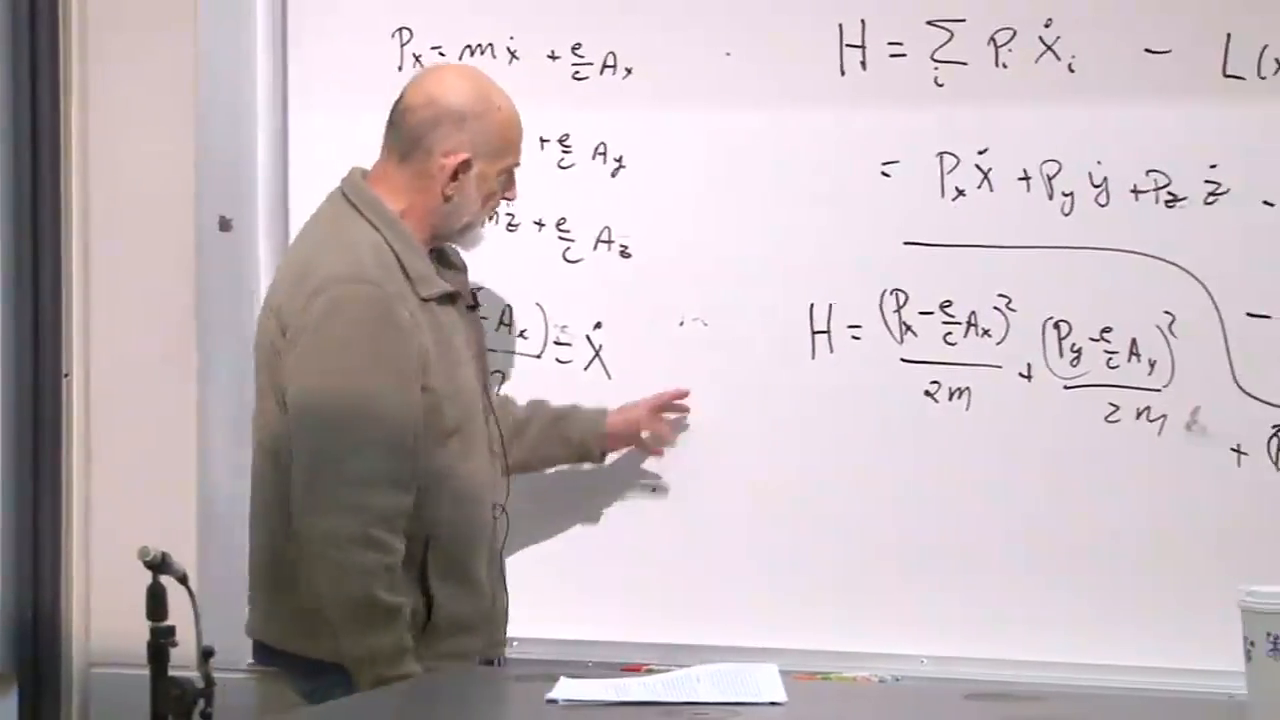
\includegraphics[width=0.86\textwidth]{lecture_10_figure_06.png}
\caption{完成的哈密顿量构造在左侧保留了三个正则动量，在右侧保留了最小耦合的平方项。}
\lectureframe{00:53:05}
\end{figure}

用正则变量写出时，这与自由粒子的哈密顿量不同。然而，用物理速度表示时，
\begin{equation}
  H=\frac{\boldsymbol{\pi}^{\,2}}{2m}
  =\frac12m\mathbf v^2.
\end{equation}
这并不矛盾。同一个数值能量由\((\mathbf x,\mathbf p)\)的不同函数表示，因此尽管能量仍等于普通的动能，哈密顿方程却不同。

由于场是静态的，\(H\)守恒。因此速率恒定。洛伦兹力使这一事实变得显而易见：
\begin{equation}
  \frac{d}{dt}\left(\frac12mv^2\right)
  =
  m\mathbf v\cdot\mathbf a
  =
  \frac{e}{c}\,
  \mathbf v\cdot(\mathbf v\times\mathbf B)
  =0.
\end{equation}
磁场改变运动方向，而不改变速度的大小。它使轨迹弯曲，但不做功。

\section{通过改变规范求解均匀场}

休息之后，再次考虑均匀场
\begin{equation}
  \mathbf B=B\hat{\mathbf z}.
\end{equation}
目标不仅仅是求解一条熟悉的轨道。而是要说明为什么选择一种规范可以使对称性计算几乎毫不费力。

\subsection{第一种规范：y 和 z 坐标为循环坐标}

取
\begin{equation}
  A_x=A_z=0,
  \qquad
  A_y=Bx.
\end{equation}
则
\begin{equation}
  L
  =
  \frac{m}{2}
  \left(\dot x^2+\dot y^2+\dot z^2\right)
  +
  \frac{eB}{c}x\dot y.
\end{equation}
坐标\(y\)和\(z\)不显式出现。它们是循环的，因此其正则动量守恒。对于\(z\)，
\begin{equation}
  p_z=m\dot z,
  \qquad
  \dot p_z=0,
\end{equation}
从而
\begin{equation}
  a_z=0.
\end{equation}
粒子沿场方向作匀速运动。

对于\(y\)，
\begin{equation}
  p_y=m\dot y+\frac{eB}{c}x,
  \qquad
  \dot p_y=0.
\end{equation}
因此
\begin{equation}
  m a_y+\frac{eB}{c}v_x=0,
  \qquad
  \boxed{m a_y=-\frac{eB}{c}v_x}.
\end{equation}

\begin{figure}[htbp]
\centering
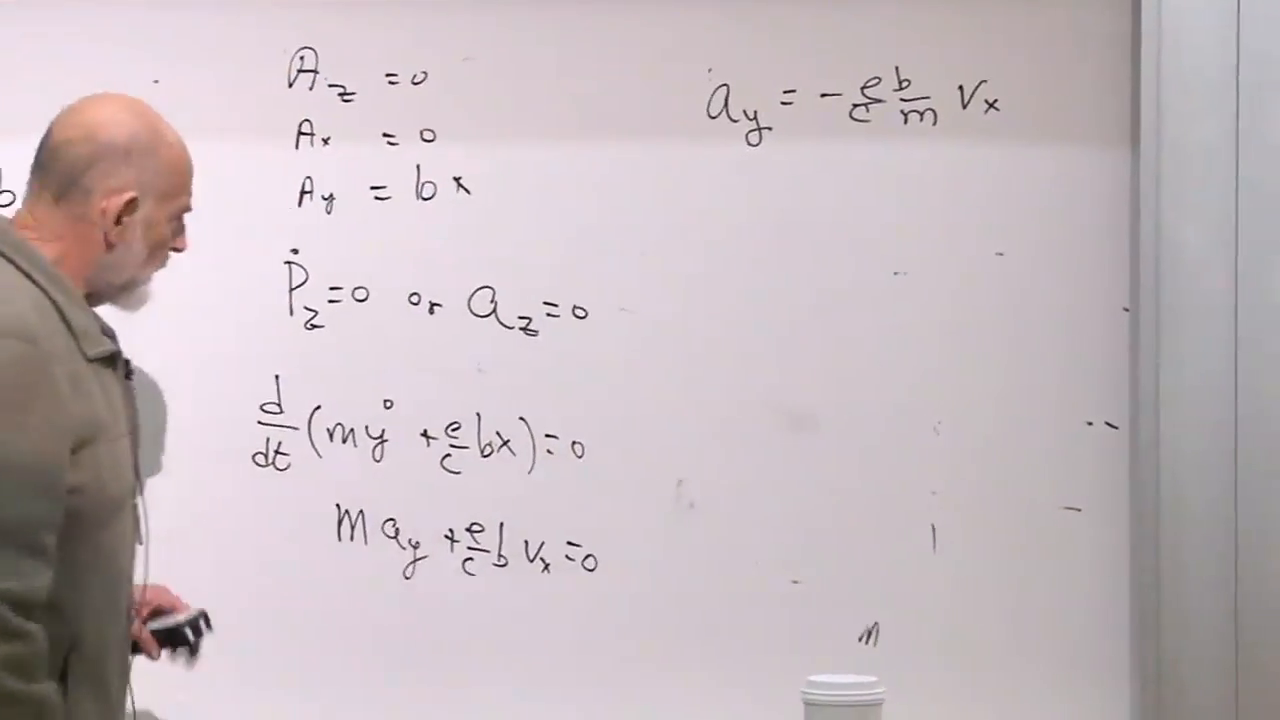
\includegraphics[width=0.84\textwidth]{lecture_10_figure_07.png}
\caption{在规范\(A_y=Bx\)中，板书记录了守恒的\(p_z\)和\(p_y\)以及由此得到的洛伦兹力\(y\)分量。}
\lectureframe{01:03:50}
\end{figure}

\subsection{第二种规范：x 坐标为循环坐标}

现在切换到
\begin{equation}
  A_x=-By,
  \qquad
  A_y=A_z=0.
\end{equation}
拉格朗日量变为
\begin{equation}
  L
  =
  \frac{m}{2}
  \left(\dot x^2+\dot y^2+\dot z^2\right)
  -
  \frac{eB}{c}y\dot x.
\end{equation}
这一次\(x\)是循环的：
\begin{equation}
  p_x=m\dot x-\frac{eB}{c}y,
  \qquad
  \dot p_x=0.
\end{equation}
因此
\begin{equation}
  \boxed{m a_x=\frac{eB}{c}v_y}.
\end{equation}
结合第一种规范的结果以及\(a_z=0\)，这恰好就是
\begin{equation}
  m\mathbf a=\frac{e}{c}\mathbf v\times B\hat{\mathbf z}.
\end{equation}

\begin{figure}[htbp]
\centering
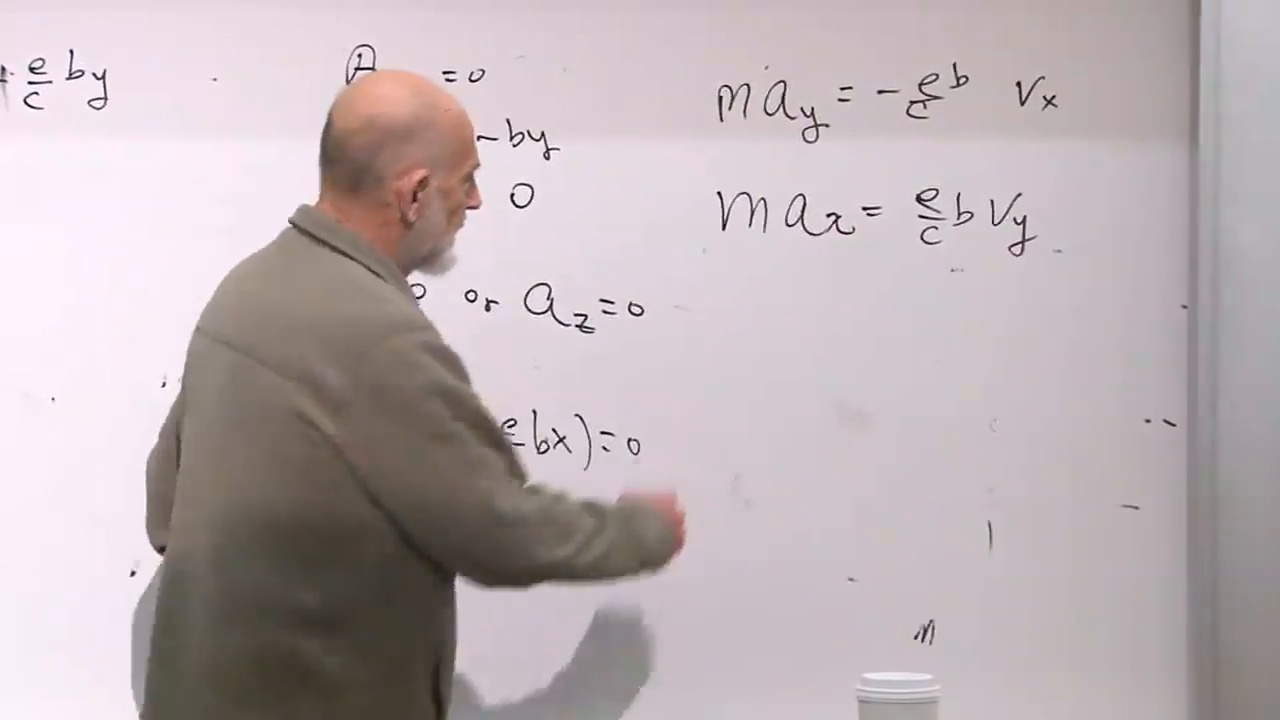
\includegraphics[width=0.84\textwidth]{lecture_10_figure_08.png}
\caption{规范切换之后，两个横向洛伦兹力分量都显现出来。每一个都是在不同规范中作为正则动量守恒定律而出现的。}
\lectureframe{01:08:05}
\end{figure}

物理的平移对称性始终存在。规范选择只改变了该对称性中哪一部分表现为普通的循环坐标。这就是为什么正则动量可以在一种规范中守恒，而在另一种规范中取不同的形式，同时可测量的加速度保持不变。

\begin{classroomqa}
\audiencequestion{正则动量的分量是规范不变的吗？它们直接具有物理意义吗？}
\lecturerresponse{不是。在\(\mathbf A\mapsto\mathbf A+\nabla S\)下，正则动量改变\((e/c)\nabla S\)。机械动量\(m\mathbf v=\mathbf p-(e/c)\mathbf A\)是规范不变的，并且直接与粒子的速度相联系。尽管如此，正则动量仍是不可或缺的，因为它是哈密顿方程和泊松括号所使用的变量。}
\end{classroomqa}

\section{均匀磁场中的轨道}

形式上的工作已经完成；现在让我们看看运动。首先假设\(v_z=0\)，因此粒子保持在\(xy\)平面内。加速度垂直于速度，且其大小恒定：
\begin{equation}
  |\mathbf a|
  =
  \frac{|e|}{mc}vB.
\end{equation}
以恒定速率运动、且具有始终垂直于其速度的恒定大小加速度的粒子，做圆周运动。

如果\(r\)是半径，则向心加速度为\(v^2/r\)。令大小相等，得到
\begin{equation}
  m\frac{v^2}{r}
  =
  \frac{|e|}{c}vB,
\end{equation}
因此
\begin{equation}
  \boxed{
  r=\frac{mcv}{|e|B}
  }.
\end{equation}
讲义首先写下了不带\(c\)的表达式，注意到与所选洛伦兹力约定不一致，然后将其恢复。\(eB\)的符号决定旋转方向；半径本身为正。

\begin{figure}[htbp]
\centering
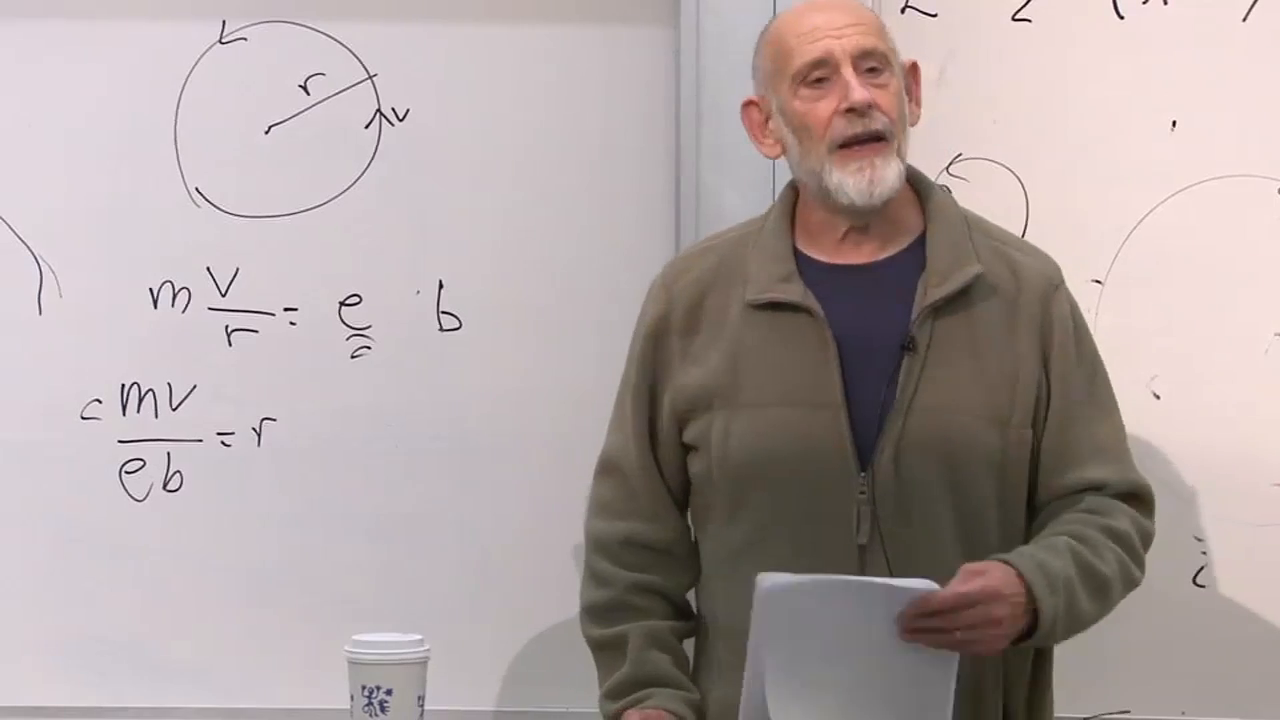
\includegraphics[width=0.84\textwidth]{lecture_10_figure_09.png}
\caption{在恢复缺失的\(c\)因子之后，圆形轨道、切向速度与半径的关系。}
\lectureframe{01:16:50}
\end{figure}

场确定了速率与半径之间的关系，但没有确定圆心。圆心可以在横向平面内的任何位置。较大的横向速率给出较大的轨道；较大的电荷或磁场给出更紧的轨道。

如果\(v_z\neq0\)，横向运动仍为圆周运动，而\(z\)均匀推进。将这两种运动结合起来，得到围绕磁场方向的螺旋线。\editorialnote{讲义分别推导了这两个要素：\(a_z=0\)和横向圆周运动。它们的组合就是所述的螺旋轨迹。}

\section{耦合从何而来？}

轨道计算促使听众回到开头。\((e/c)\mathbf A\cdot\mathbf v\)这一项是事先就知道的吗？诚实的回答是，存在若干逻辑上自洽的出发点。

\begin{classroomqa}
\audiencequestion{我们只是知道磁拉格朗日量并把它写下来吗？}
\lecturerresponse{就本次讲述而言，是的：写下速度线性耦合并研究它。从该项出发，人们会发现规范不变性，然后发现方程中的旋度组合表现为磁场。人们也可以从观测到的洛伦兹力出发并寻找作用量，或者从现代对规范不变性的要求出发。历史上，这些片段是以不那么直接的顺序被发现的。}
\end{classroomqa}

还有一个有用的检验，用来判断一个提议的拉格朗日量是否支持通常的哈密顿构造。方程
\begin{equation}
  p_i=\frac{\partial L}{\partial\dot x_i}
\end{equation}
必须对速度可逆，至少在这里所考虑的正则系统中如此。用更精确的语言说，速度黑塞矩阵
\begin{equation}
  \frac{\partial^2L}
       {\partial\dot x_i\,\partial\dot x_j}
\end{equation}
必须非奇异。对于这个粒子，它简单地就是\(m\delta_{ij}\)，因此勒让德变换是明确的。

\begin{classroomqa}
\audiencequestion{是什么使一个提议的拉格朗日量合法？}
\lecturerresponse{对于这里所发展的普通力学，它应当给出明确的运动方程，并允许在用动量解出速度之后得到唯一的哈密顿量。奇异拉格朗日量确实出现在规范场论中，但处理它们的约束需要超出本课程的机制。}
\end{classroomqa}

\begin{classroomqa}
\audiencequestion{规范对称性本身会给出守恒量吗？}
\lecturerresponse{仅从规定背景下的粒子问题不能。要恰当地讨论相应的守恒定律，必须把电磁场包括在动力学变量之中。在完整的场论中，规范不变性与电荷守恒相联系，但这需要场的作用量和麦克斯韦方程。}
\end{classroomqa}

\section{固定背景与麦克斯韦动力学}

到目前为止，没有任何东西告诉电磁场如何演化。场是作为固定背景给出的，而问题只是：给定\(\mathbf E\)和\(\mathbf B\)，粒子如何运动？

\begin{classroomqa}
\audiencequestion{这与麦克斯韦方程有什么关系？}
\lecturerresponse{要推导麦克斯韦方程，必须加入电磁场自身的作用量，并对场以及粒子轨迹进行变分。耦合项\((e/c)\int\mathbf A\cdot d\mathbf x\)是完整作用量的一部分。当背景保持固定时，场项不影响粒子变分，但当场本身成为动力学变量时，它是必不可少的。}
\end{classroomqa}

在经典情形下，人们可以忽略作用量形式，直接假定
\begin{equation}
  m\mathbf a=\frac{e}{c}\mathbf v\times\mathbf B.
\end{equation}
对于检验粒子的力学而言，这是一个完全有意义的微分方程。但拉格朗日结构和哈密顿结构在量子力学中变得不可或缺，因为在那里矢量势直接进入理论。

\section{磁单极子与细螺线管图像}

如果
\begin{equation}
  \nabla\cdot\mathbf B\neq0?
\end{equation}
那么\(\mathbf B\)就不能处处由一个光滑的矢量势表示，因为每个旋度的散度都为零。本章所用的简单整体构造失效了。

讲座通过设想一根极长、极细的条形磁铁或螺线管来说明这个问题。靠近一端，而另一端被带到任意远处时，外部场类似于一个磁极的场。返回的磁通并没有消失；它被限制在细管内部。如果把这根管子做得理想化且不可观测，它就会扮演附着在表观磁单极子上的弦的角色。

\begin{figure}[htbp]
\centering
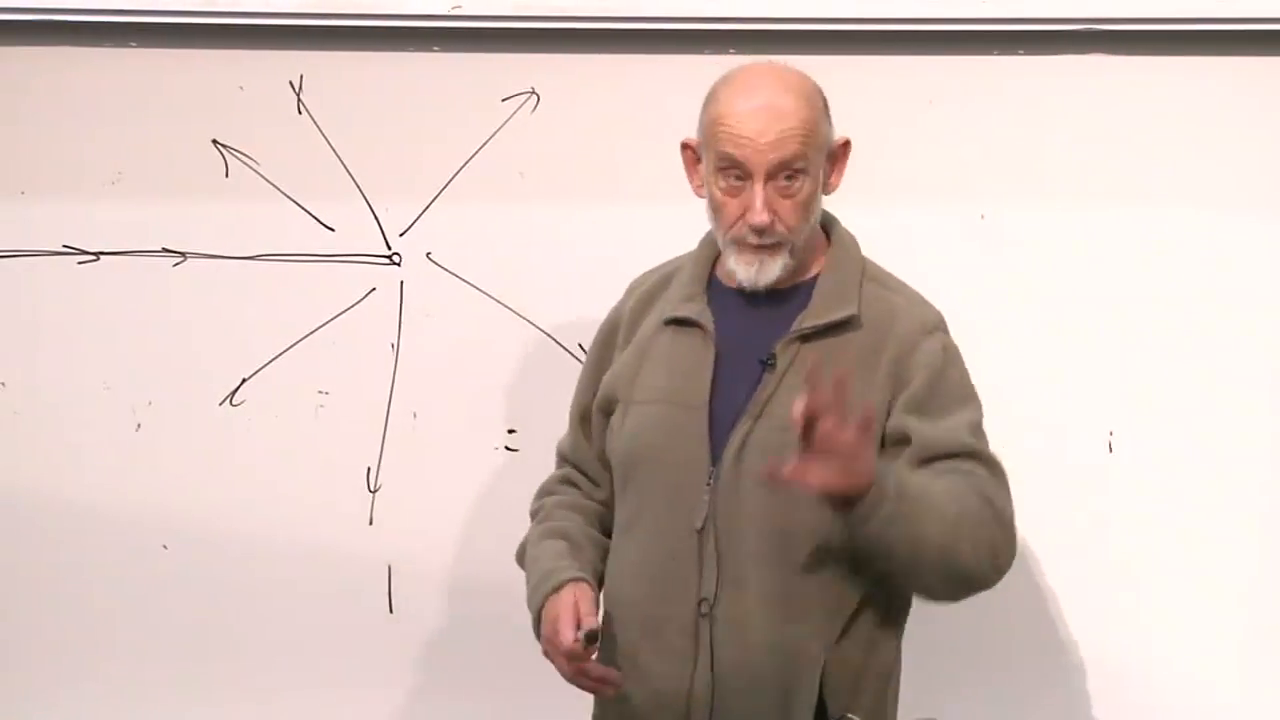
\includegraphics[width=0.84\textwidth]{lecture_10_figure_10.png}
\caption{黑板上的细螺线管图像：场线从一个表观磁极散开，而返回的磁通被限制在狭窄的管中。}
\lectureframe{01:27:35}
\end{figure}

在普通经典电磁学中，把固定磁通挤压到趋于零的横截面上会使场强和场能不断增大。讲座故意用关于无限能量的夸张回答来强调，现实的磁单极子需要新物理，而不只是把普通螺线管做得越来越细。在量子理论中，经过适当量子化的通量管可以在其核心之外变得不可观测；这就是狄拉克弦构造背后的思想，尽管完整的磁单极子理论超出了本课程的范围。

\begin{classroomqa}
\audiencequestion{一个点粒子可以具有磁矩。那是磁单极子吗？}
\lecturerresponse{不是。磁矩是偶极子：它具有大小相等、符号相反的磁极性质。磁单极子则会携带一个净磁荷。切开普通磁铁并不能分离出它的磁极；每一块都会获得自己的北极和南极。}
\end{classroomqa}

\begin{classroomqa}
\audiencequestion{分离两端之困难是否类似于夸克禁闭？}
\lecturerresponse{这是一个有用的类比。把禁闭的夸克拉开会在普通观测中得不到孤立的夸克；连接它们的场会产生新的束缚客体。这里并不是在认定这些机制相同，但由不可避免的通量结构连接端点的图像是相似的。}
\end{classroomqa}

讲座的结论是谨慎的。磁单极子不属于推导中所用的普通经典理论，但许多高能理论包含它们。如果它们作为基本粒子存在，预计会涉及远超课堂力学范围的能标。

\section{哈密顿的另一套代数与未完成的话题}

最后一个听众提问问的是哈密顿的四元数。它们在历史上与哈密顿力学是分开的。哈密顿寻求一种代数，能在三维旋转中扮演某种类似于复数在平面旋转中所扮演的角色。其结果使用三个虚数单位\(i,j,k\)，满足
\begin{equation}
  i^2=j^2=k^2=ijk=-1,
\end{equation}
并且，例如，
\begin{equation}
  ij=k,
  \qquad
  ji=-k.
\end{equation}
单位四元数提供了三维旋转的一种高效表示。在量子力学中，同样的代数结构可以用泡利矩阵表示，并配上普通虚数单位的适当因子。这种联系是真实的，但它并不是本课程所发展的正则动量或哈密顿量的起源。

最后被要求讲的主题是混沌。已经没有时间展开它了。讲座最后回指已经建立起来的工具：动力学是相空间中沿轨道的运动，而这种语言正是研究规则行为和混沌行为的起点。经典力学的形式结构已经足够完整，听众可以从那里继续下去。
